%%%%%%%%%%%%%%%%%%%%%%%%%%%%%%%%%%%%%%%%%%%%%%%%%%%%%%%%%%%%%%%%%%%%%%%%%%%%%
%
% This is a LaTeX file for an A3 poster.
%
%%%%%%%%%%%%%%%%%%%%%%%%%%%%%%%%%%%%%%%%%%%%%%%%%%%%%%%%%%%%%%%%%%%%%%%%%%%%%

%%%%%%%%%%%%%%%%%%%%%%%%%%%%%%%%%%%%%%%%%%%%%%%%%%%%%%%%%%%%%%%%%%%%%%%%%%%%%
%%%%%%%%%%%%%%%%%%%%%%%%%%%%%%%%%%%%%%%%%%%%%%%%%%%%%%%%%%%%%%%%%%%%%%%%%%%%%
%
% Asymptotic behavior of solutions to the generalized Becker-Döring
% equations for general initial data.
%
% Poster for the HYKE-3 meeting in Rome, 13-15 April 2005.
%
%%%%%%%%%%%%%%%%%%%%%%%%%%%%%%%%%%%%%%%%%%%%%%%%%%%%%%%%%%%%%%%%%%%%%%%%%%%%%
%%%%%%%%%%%%%%%%%%%%%%%%%%%%%%%%%%%%%%%%%%%%%%%%%%%%%%%%%%%%%%%%%%%%%%%%%%%%%

\documentclass[american]{article}
% To modify the size of the page:
\usepackage[dvips,paperwidth=34in,paperheight=44in,landscape,centering,left=3.0cm,right=3.0cm,top=3.0cm, bottom=3.0cm]{geometry}
\usepackage{babel}
\usepackage{multicol}
\usepackage[utf8]{inputenc}
\usepackage{color,xcolor}
\usepackage{float}
\usepackage{amsmath, amsthm, amsfonts}
\usepackage{graphicx}           % Include figure files.
\usepackage{anyfontsize}
\usepackage{setspace}
\usepackage{lipsum}
% Colors
% -------
\usepackage[immediate]{silence}
\WarningFilter[temp]{latex}{Command} % silence the warning
\definecolor{azulcielo}{RGB}{227,243,248}

\newcommand\Mark[1]{\textsuperscript#1}
\pagestyle{empty}

\def\to{\rightarrow}
\usepackage{geometry}
\usepackage{layout}
\usepackage{url}
\usepackage[pdftex, pdfborderstyle={/S/U/W 0}]{hyperref}
\usepackage{csquotes}
\usepackage[backend=biber, style=ieee,language=auto]{biblatex}
\addbibresource{bibliography.bib}

\graphicspath{{media/images/}}
\DeclareGraphicsExtensions{.jpeg,.png,.jpg}
\usepackage{sectsty}
%\usepackage[breaklinks]{hyperref}
\sffamily
\sectionfont{\fontsize{50}{72}\selectfont}
%\renewcommand{\familydefault}{\sfdefault}
\usepackage{libertine}
%\usepackage{newtxtext}
%\usepackage{libertinust1math}
\usepackage{newtxmath}
\usepackage[T1]{fontenc}

\newcommand\pd[2]{\frac{\partial #1}{\partial #2}}
\newcommand\inte{\int_{\Omega^e}}
\newcommand\pinte{\int_{\partial\Omega^e}}
\newcommand\ve[1]{\mathbf{#1}}

\urlstyle{sf}
\usepackage{titlesec}
\titlespacing{\section}{0pt}{1ex}{1ex}
% ===========================================================================
\usepackage{array}
\title{}
\author{}
\date{}

\begin{document}
%\maketitle

\begin{center}
  \begin{minipage}{.2\linewidth}
  %\qquad\qquad
    
\includegraphics[width=\linewidth]{media/images/oden-logo-2019.png}
    ~\vfill
    ~\vfill
  \end{minipage}
  %&
  %\vspace{-0.75cm}
  \begin{minipage}{.6\linewidth}
    \begin{center}
       \textsf{\textbf{{\fontsize{65}{108}\selectfont  Developing a Compound Flooding Model using the Discontinuous Galerkin Method}}}\\\vspace{1cm}
       \textrm{\fontsize{40}{48}\selectfont Chayanon (Namo) Wichitrnithed, Eirik Valseth, Clint Dawson \\\vspace{5mm} \textit{The Oden Institute for Computational Engineering and Sciences at the University of Texas at Austin} \vspace{5mm} }
    \end{center}
  \end{minipage}
  %&
  \hspace{.03\linewidth}
    \begin{minipage}{.16\linewidth}
    
\includegraphics[width=\linewidth]{media/planet.png}
    ~\vfill
    ~\vfill
  \end{minipage}
\end{center}

%\vspace{0.5cm}

\hrulefill
\vspace{10mm}
% ---------------------------------------------------------------------------
\fontsize{30}{36}\selectfont
\setlength{\columnsep}{1cm}
\vspace{-1.00cm}
\begin{multicols}{3}
% ---------------------------------------------------------------------------
% En caso de no poner resumen se comenta la siguiente sección
% ---------------------------------------------------------------------------
\noindent

\section*{Introduction}

\begin{center}
  \vspace{5mm}
  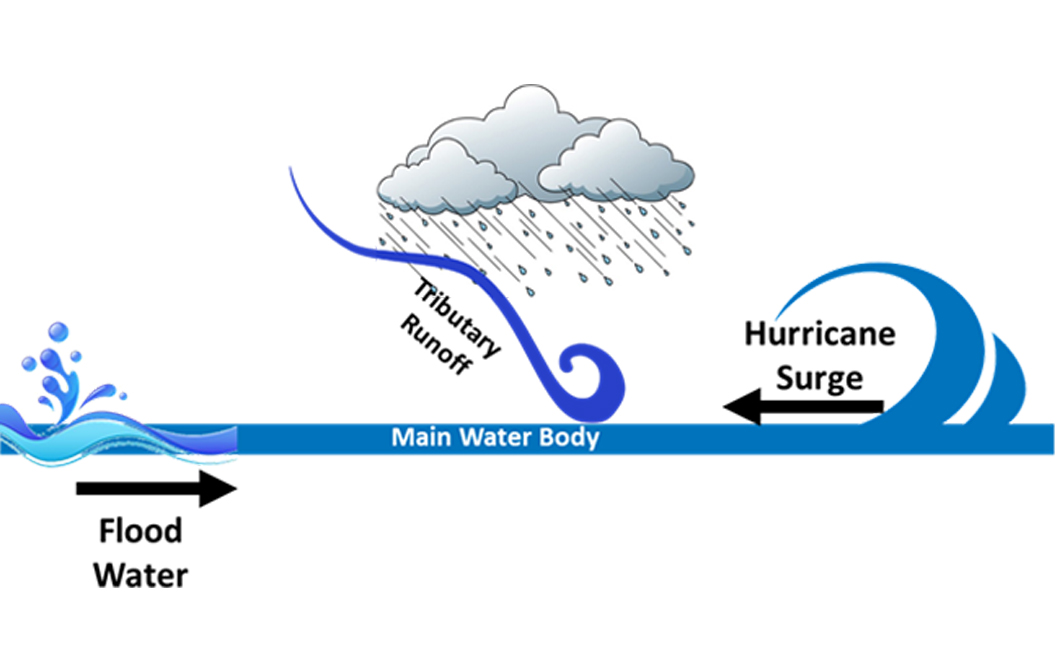
\includegraphics[width=0.85\linewidth]{media/compound_flooding.jpg} \\
  \textbf{Figure 1:} Components of compound flooding [1].
\end{center}
Compound flooding is a complex phenomena that arises when flooding sources such as storm surge, rainfall and river discharge occur simultaneously. The combined effect of these sources can be devastating, as most notably seen in Houston area during Hurricane Harvey, where storm surges prevented drainage of rainfall runoff (Figure 1). This interdependency makes it difficult to simulate compound flooding because the model has to be able to combine these sources in a nonlinear way.

Regular simulations are usually done with the Advanced Circulation Model (ADCIRC), a computer program that discretizes the fluid on a 2D finite element mesh. However, it is difficult to add source terms that account for parts of compound flooding, in this case rainfall. Moreover, the continuous Galerkin method (CG) used in ADCIRC does not guarantee mass conservation in each element which can lead to inaccuracies when source terms are added.
Due to these limitations, we test the effect of incorporating rainfall and river discharge into the Discontinuous Galerkin Shallow Water Equation model (DG-SWEM), a model based on ADCIRC that uses the discontinuous Galerkin method (DG).

\hrulefill

\section*{Model}
\noindent DG-SWEM uses the shallow water equations (SWE) which are an approximate model for a thin (relative to depth) layer of water in two dimensions. The continuity equation in this case is simply
\begin{align*}
  \pd{\zeta}{t} + \pd{}{x} (Hu) + \pd{}{y} (Hv) = {\color{red} S(t,x,y)}
\end{align*}
where $\zeta$ is the water elevation, $H$ is the total height of the water column, $u$ and $v$ the velocities in $x$ and $y$ directions, and $\color{red} S$ is the rainfall per unit area. Rainfall can of course vary in time and among different parts of the domain, but in this test we use constant rainfall.

\begin{center}
  \vspace{5mm}
  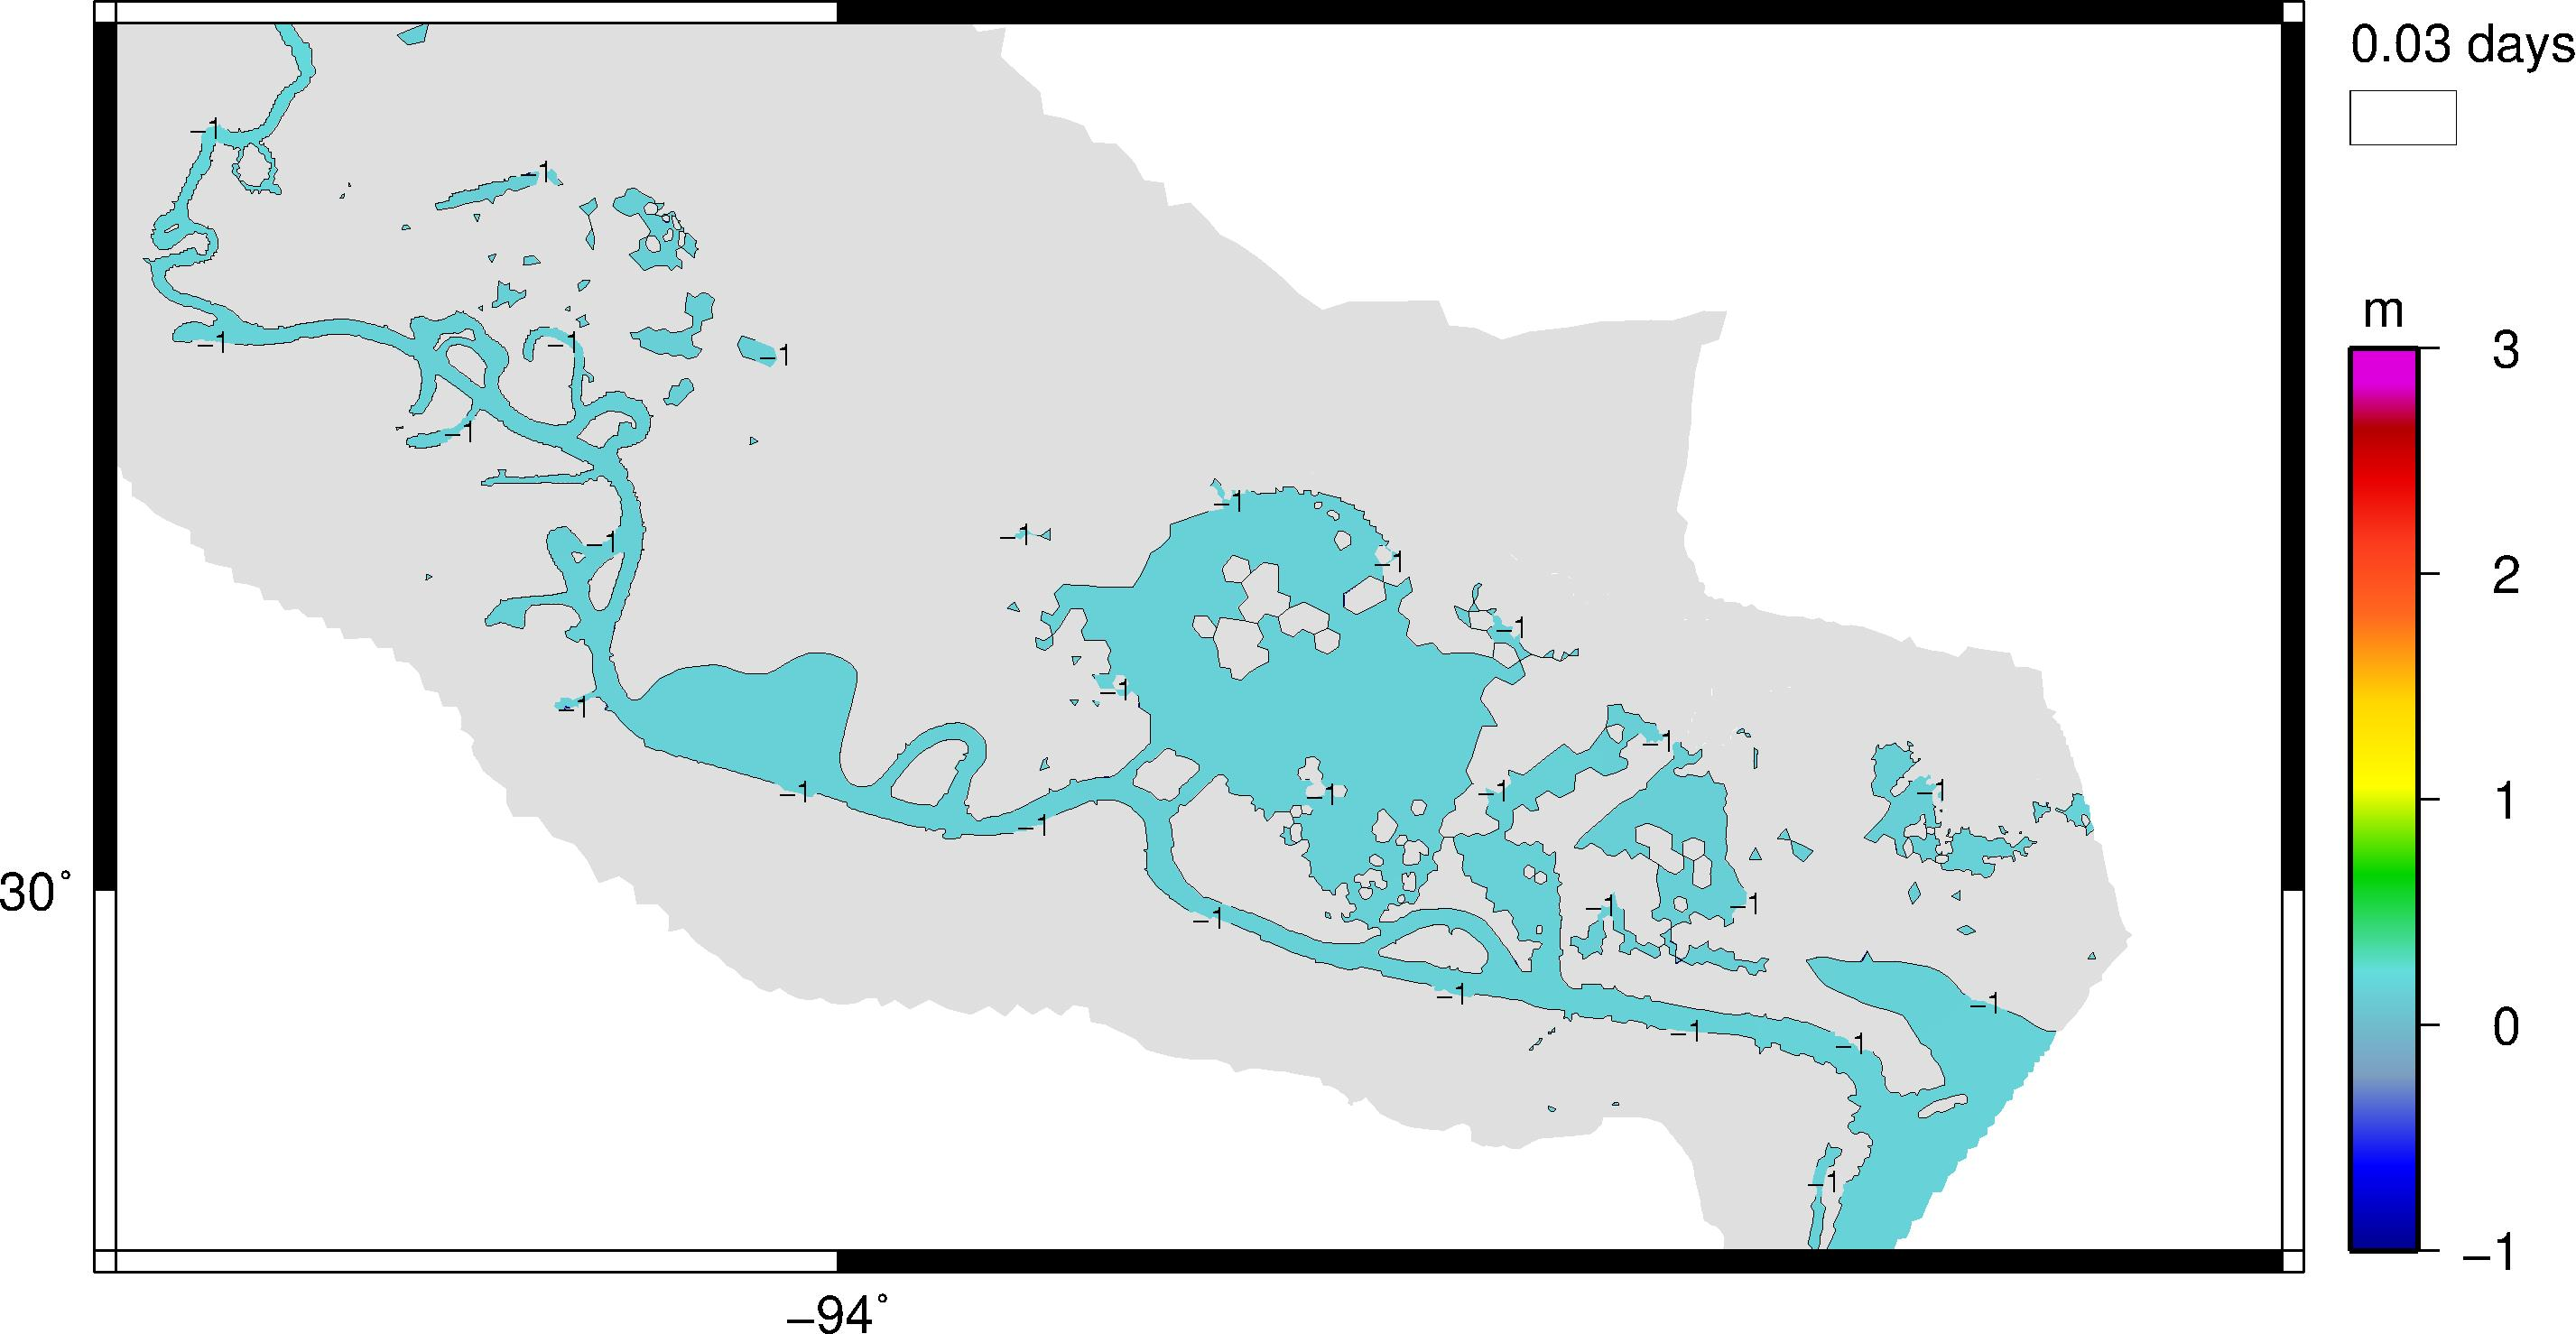
\includegraphics[width=0.95\linewidth]{media/grid.jpg}
  \textbf{Figure 2}: Finite element mesh of the Neches river
\end{center}

The test case is the Neches River shown in Figure 2, triangulated with 62,075 nodes. We model the flow during Hurricane Harvey, where rainfall and river discharge occur upstream and travel down the river.

\hrulefill
\section*{Method}
\noindent The DG method differs from CG in that it enforces the weak form on each individual element and the solution is allowed to be discontinuous across elements. This effectively guarantees that water elevation is conserved in each element, i.e. the net change is only due to inflow and outflow. In mathematical terms, the weak form for the continuity equation on element $\Omega^e$ is
\begin{align*}
  \inte \pd{\zeta}{t} w - \inte \nabla w \cdot \ve{F} + \pinte w \ve{\widehat{F}} \cdot \ve{n}  = \inte w S.
\end{align*}
Here, $\partial \Omega^e$ is the element boundary, $\ve{F}$ is the vector $[uH, vH]^T$, $w$ is the test function on $\Omega^e$, and $\ve{\widehat{F}}$ is the appropriate numerical flux (the Roe flux is used here).
\begin{center}
  \vspace{5mm}
    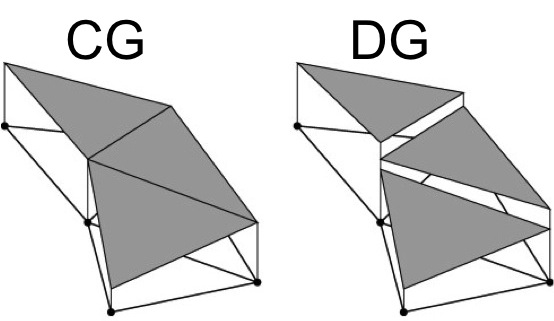
\includegraphics[width=0.55 \linewidth]{media/DG_CG.jpg} \\
    \textbf{Figure 3:} An comparison of linear continuous- and discontinuous Galerkin elements [2]. In DG, the solution doesn't need to match at the nodes.
\end{center}
Upstream river discharge is added by supplying the flow rates $u$ and $v$ to the numerical flux at the corresponding element boundaries.
Solving this system yields a system of ODEs which we then solve using the second order Strong Stability Preserving Runge-Kutta scheme (SSPRK).
Finally, the solution at the nodes is obtained by averaging the values of discontinuous solutions from the neighboring elements.


\section*{Results and Discussion}
\noindent We ran DG-SWEM on the Neches domain with 1 inch of rain per hour, constant throughout the whole domain. The simulation was run on 128 CPU cores at a time step of 0.1 seconds for 6 simulation days, which took around 6 hours in real time. A plot of water elevation at day 6 is given in Figure 4. As can be seen, the flow is compounded by the river discharge from the top left corner as well as rainfall on the rest of the domain.
\begin{center}
    \vspace{0.5cm}
    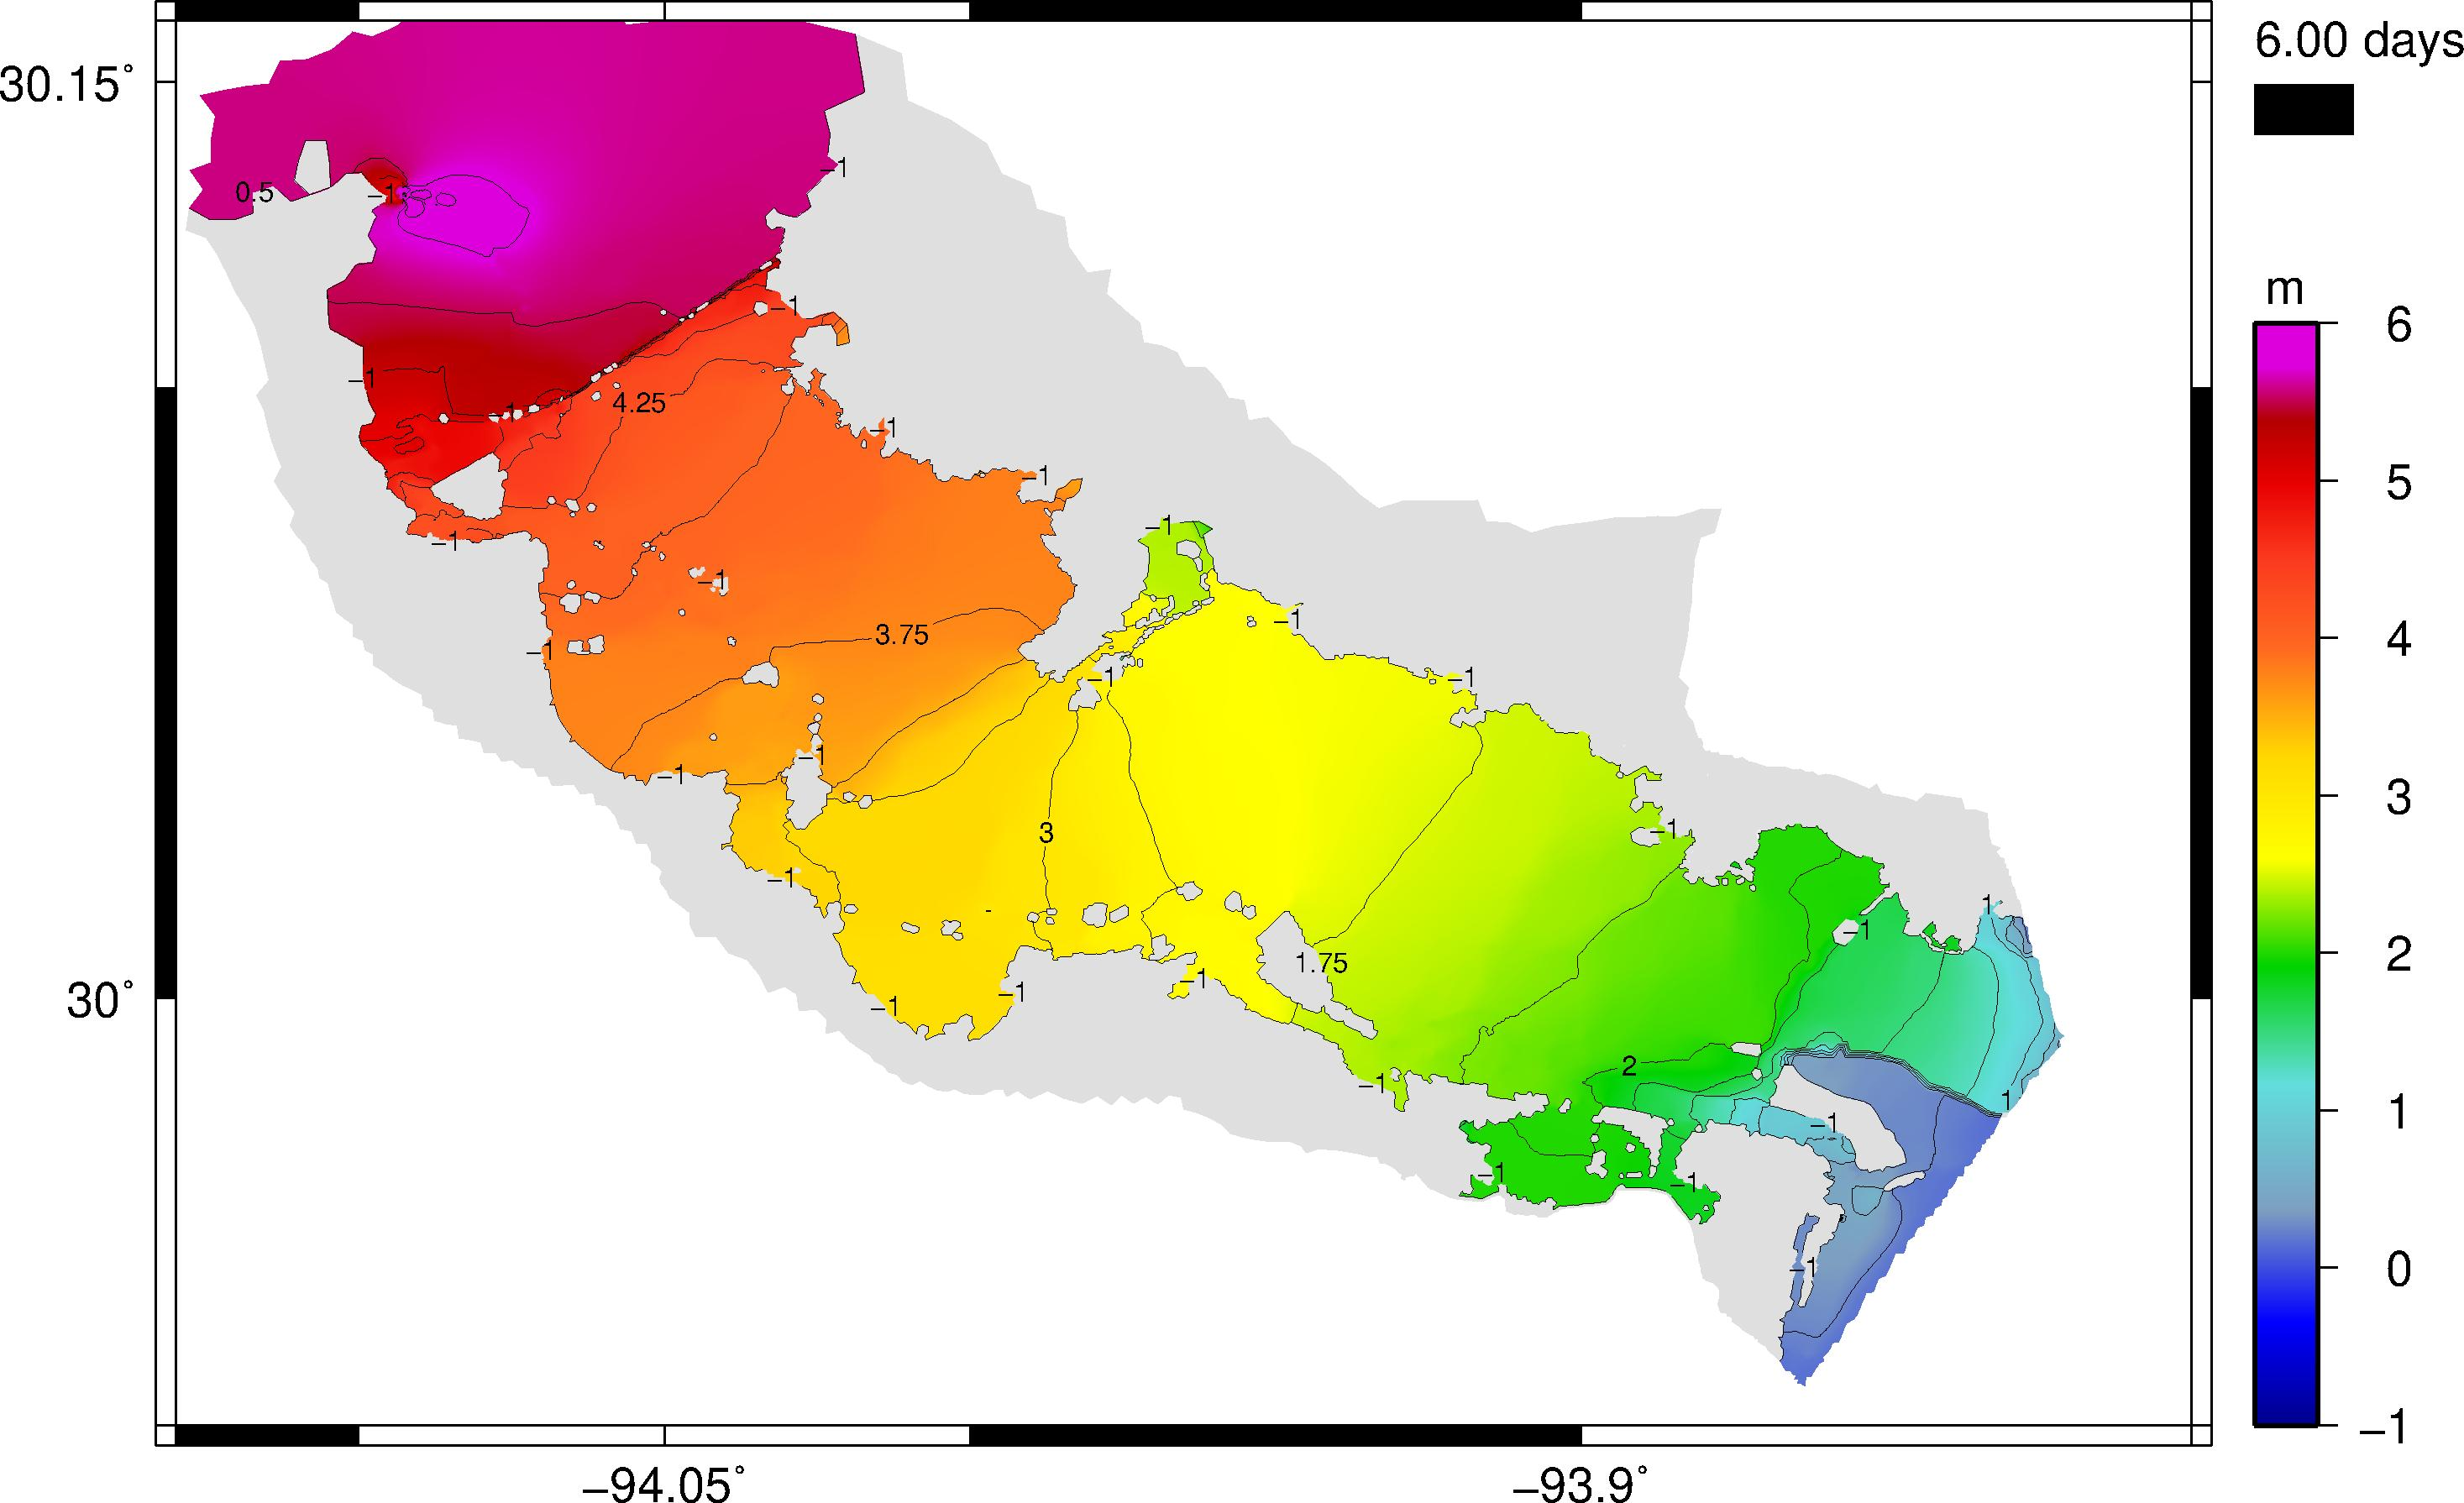
\includegraphics[width=0.95 \linewidth]{media/rain.jpg}
    \textbf{Figure 4:} Water elevation of the Neches river on the 6th day.
\end{center}
We also plot below the water elevation time series for simulations with and without rainfall in Figure 5. These are computed at two recording stations in the domain.
\begin{center}
    \vspace{0.5cm}
    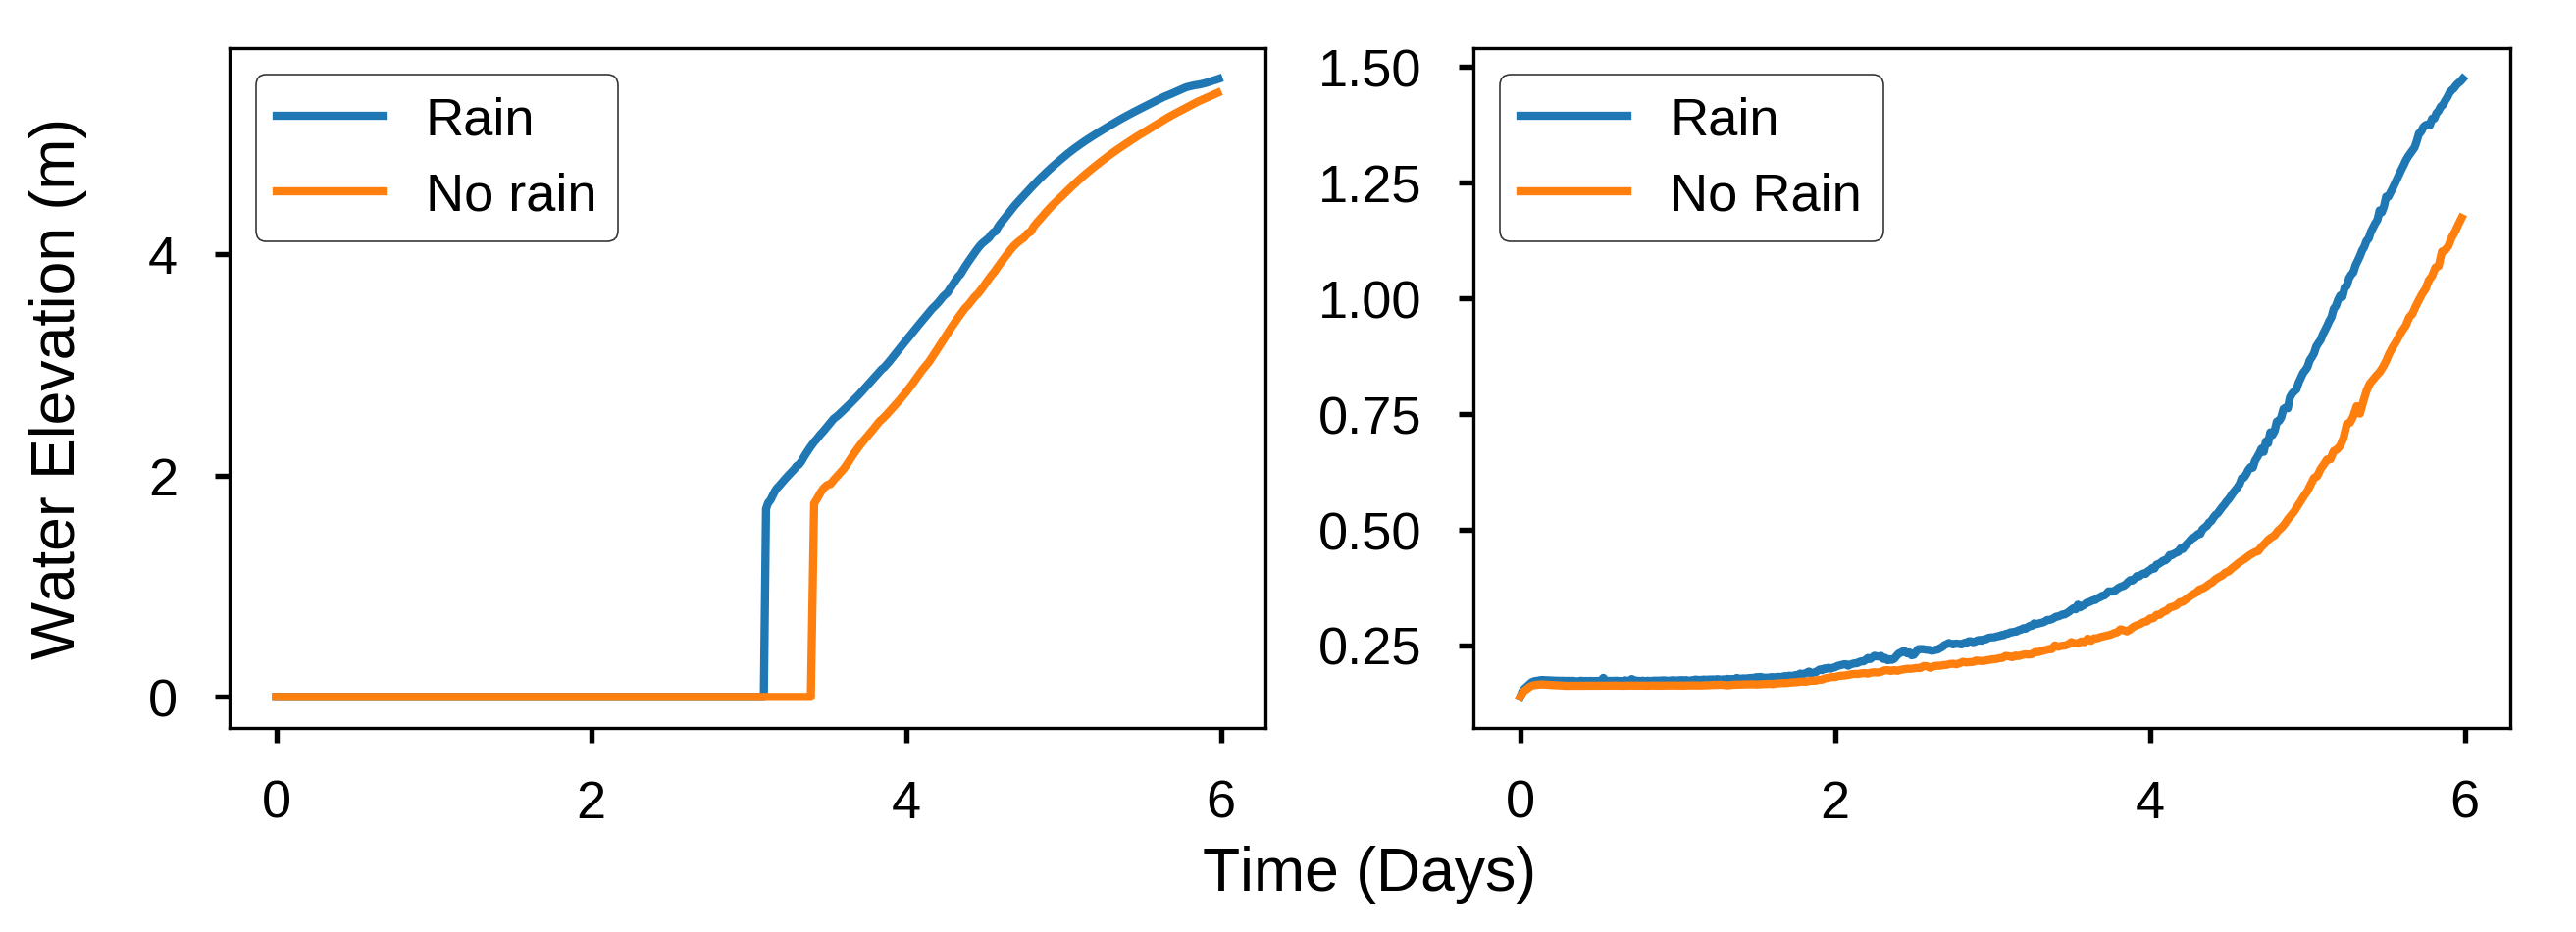
\includegraphics[width=0.95 \linewidth]{media/double.png}
    \textbf{Figure 5}: Water elevation data from the simulation measured at Rainbow Bridge (right) and at Salt Water Barrier (left).
\end{center}

As a first test, these results look reasonable; for instance, the salt barrier location becomes wet slightly faster with rain and produces a higher surface elevation but in a similar pattern compared to the case without rain. Following this, we aim to test the model on bigger hurricane datasets and perform verification on the results.


\begin{thebibliography}{2}
\bibitem{compound}
  Ask an expert: A coastal flood modeler explains compound flooding. (2021). Retrieved from \url{https://texaswaternewsroom.org/articles/a_coastal_flood_modeler_explains_compound_flooding.html}
\bibitem{dg}
  Discontinuous Galerkin finite element methods. Retrieved from \url{https://mathstats.uncg.edu/applied/dgfiniteelement/}
\end{thebibliography}
% \renewcommand{\bibfont}{\fontsize{20}{20}\selectfont}
% \nocite{*}
% \printbibliography



\end{multicols}

\end{document}
